\documentclass{beamer}
% September 2014 
% Author: Dr Rachid Hourizi and Dr. Michael Wright 
% Department of Computer Science, University of Bath
\usepackage{listings}
\usetheme{Boadilla} 
\usepackage{fixltx2e}
\usepackage{hyperref}
\lstset{language=Java,,
	basicstyle=\ttfamily\small,
           keywordstyle=\color{blue}\ttfamily,
           stringstyle=\color{red}\ttfamily,
           commentstyle=\color{gray}\ttfamily,
          breaklines=true}

\begin{document}

\AtBeginSection[]{
  \begin{frame}
  \vfill
  \centering
  \begin{beamercolorbox}[sep=8pt,center,shadow=true,rounded=true]{title}
    \usebeamerfont{title}\insertsectionhead\par%
  \end{beamercolorbox}
  \vfill
  \end{frame}
}

\title{CM 10227: Lecture 9}
\author{Dr Rachid Hourizi and Dr Michael Wright}
\date{\today}
\frame{\titlepage}

\begin{frame} 
\begin{center}
\textbf{Resources}
\end{center}
\begin{itemize}
\item More help with this course
\begin{itemize}
\item Moodle
\item E-mail - programming1@lists.bath.ac.uk
\end{itemize}
\item Online C and Java IDE
\begin{itemize}
\item https://www.codechef.com/ide
\item Remember to select Java from the drop down menu.
\end{itemize}
\item Books
\begin{itemize}
\item Java by Dissection (Free pdf online)
\item The Java Tutorial (https://docs.oracle.com/javase/tutorial/)
\end{itemize}
\end{itemize}
\end{frame}

\begin{frame} 
\begin{center}
\textbf{Resources}
\end{center}
\begin{itemize}
\item The places that you can get additional support if you are finding the pace of the course a little fast now include
\begin{itemize}
\item A labs (Continued from week 1)
\item B labs 
\item ... Wednesday 11:15-13:05 EB0.7
\item ... Fridays 17:15 to 19:15 in CB 5.13)
\item The Drop in Session 
\item ... booked 20 min appointments
\item ... Friday 11.15-13.05 1E 3.9
\item PAL sessions (Mondays 14:15 to 15:05 1E 3.9)
\end{itemize}
\end{itemize}
\end{frame}

\begin{frame}
\begin{center}
\textbf{Last Week}
\end{center} 
\begin{itemize}
\item Interfaces 
\item Abstract Classes
\end{itemize}
\end{frame}

\begin{frame}
\begin{center}
\textbf{This week }
\end{center}
\begin{itemize}
\item Errors
\item Exceptions
\item Style : Writing Better Code
\end{itemize}
\end{frame}

\begin{frame}
\begin{center}
\textbf{Overview}
\end{center}
\begin{itemize}
\item Defensive programming.
\item Anticipating that things could go wrong.
\item Exception handling and throwing. 
\item Error reporting.
\end{itemize}
\end{frame}

\begin{frame}
\begin{center}
\textbf{Robustness of Code}
\end{center}
\begin{itemize}
\item Robustness is the ability of a computer system to... 
\bigskip
\item ... cope with errors during execution 
\item ... and cope with erroneous input.
\end{itemize}
\end{frame}

\begin{frame}
\begin{center}
\textbf{Example Programming Errors}
\end{center}
\begin{itemize}
\item Some problems really should be addressed by the programmer during coding
\end{itemize}
\begin{itemize}
\item Incorrect implementation.
\begin{itemize}
\item does not meet the specification.
\end{itemize}
\item Inappropriate object request. 
\begin{itemize}
\item e.g. invalid index.
\end{itemize}
\end{itemize}
\end{frame}

\begin{frame}[fragile]
\begin{center}
\textbf{Guarding}
\end{center}
\begin{itemize}
\item Some of those problems can, in turn be addressed with appropriate conditional statements
\end{itemize}
\begin{block}{}
\begin{lstlisting}
if (number is above zero){
    calculate corresponding Fibonacci number
}
\end{lstlisting}
\end{block}

\begin{block}{}
\begin{lstlisting}
if (index is within bounds){
    return element with that index from Array
}
\end{lstlisting}
\end{block}
\end{frame}

\begin{frame}
\begin{center}
\textbf{Guarding}
\end{center}
\begin{itemize}
\item This kind of conditional statement that is used to decide whether a branch of the program will execute is called a
guard
\item Strictly, a guard is the boolean expression that must evaluate to true if the `guarded' block of code is to
execute
\item You should certainly use guards in your programs
\end{itemize}
\end{frame}

\begin{frame} 
\begin{itemize}
\item (Arguably), however, not all errors are programmer errors
\item Errors often arise from the environment: 
\begin{itemize}
\item Incorrect URL entered.
\item Network interruption.
\end{itemize}
\item File processing is particular error-prone:
\begin{itemize}
\item Missing files.
\item Lack of appropriate permissions.
\end{itemize}
\end{itemize}
\end{frame}

\begin{frame} 
\begin{center}
\textbf{Defensive Programming}
\end{center}
\begin{itemize}
\item Client-server interaction.
\begin{itemize}
\item Should a server assume that clients are well-behaved? 
\item Or should it assume that clients are potentially hostile?
\end{itemize}
\item Significant differences in implementation required.
\end{itemize}
\end{frame}

\begin{frame}
\begin{center}
\textbf{Issues to be Addressed}
\end{center}
\begin{itemize}
\item How much checking by a server on method calls? 
\item How to report errors?
\item How can a client anticipate failure?
\item How should a client deal with failure?
\end{itemize}
\end{frame}

\begin{frame}
\begin{center}
\textbf{An example: The AddressBook Project}
\end{center}
\begin{itemize}
\item Create an Online AddressBook object
\bigskip
\item Try to remove an entry.
\item A runtime error results.
\item Whose fault is this?
\end{itemize}
\end{frame}

\begin{frame}
\begin{center}
\textbf{An example: The AddressBook Project}
\end{center}
\begin{itemize}
\item Anticipation and prevention are preferable to apportioning blame.
\end{itemize}
\end{frame}

\begin{frame}
\begin{center}
\textbf{Arguments And Errors}
\end{center}
\begin{itemize}
\item Arguments represent a major vulnerability for a server object.
\item Constructor arguments initialize state.
\item Method arguments often contribute to behaviour.
\item Argument checking is one defensive measure.
\end{itemize}

\end{frame}

\begin{frame}[fragile]
\begin{center}
\textbf{Checking the Key}
\end{center}
\begin{block}{}
\begin{lstlisting}
public void removeDetails(String key) {
  if (keyInUse(key)) { 
    ContactDetails details = book.get(key);
    book.remove(details.getName());
    book.remove(details.getPhone());
    numberOfEntries --; 
  }
}
\end{lstlisting}
\end{block}
\end{frame}

\begin{frame}
\begin{center}
\textbf{Aside : i - -  and - - i}
\end{center}
\begin{itemize}
\item Note the use of the decrement operator on the previous slide\\  (double minus or - -)
\item The use of that decrement operator after the variable (numberOfEntries) means decrement the value \textbf{after} any operations involving that variable have concluded
\item Putting the decrement operator \textbf{before} the variable name (- -i) would mean decrement and then perform those operations.
\bigskip
\item Similarly, the increment operator (++) can be used before the variable (increment then use, ++i) or afterwards (i++, use then increment)
\end{itemize}
\end{frame}

\begin{frame}[fragile]
\begin{center}
\textbf{Aside : i - -  and - - i}
\end{center}
\begin{block}{}
\begin{lstlisting}
public static void main (String[] args) {
    int i = 3;
    i++;
    System.out.println(i);
    ++i;			   
    System.out.println(i);
    System.out.println(++i); 
    System.out.println(i++); 
    System.out.println(i);
}
\end{lstlisting}
\end{block}
\begin{center}
what is printed ?
\end{center}
\end{frame}

\begin{frame}[fragile]
\begin{center}
\textbf{Aside : i - -  and - - i}
\end{center}
\begin{block}{}
\begin{lstlisting}
4
5
6
6
7
\end{lstlisting}
\end{block}
\end{frame}

\begin{frame}[fragile]
\begin{center}
\textbf{Aside : i - -  and - - i}
\end{center}
\begin{block}{}
\begin{lstlisting}
public static void main (String[] args) {
    int i = 3;
    i++;
    System.out.println(i); // prints 4
    ++i;			   
    System.out.println(i);  // prints 5
    
    // increments before the print so prints 6
    System.out.println(++i); 
    
    // increments *after* the print so prints 6
    System.out.println(i++); 
    
    System.out.println(i); // prints 7
}
\end{lstlisting}
\end{block}
\end{frame}

\begin{frame} 
\begin{center}
\textbf{Server Error Reporting Questions:}
\end{center}
\begin{itemize}
\item How to report illegal arguments?
\item To the user? 

\begin{itemize}
\item Is there a human user? 
\item Can they solve the problem?
\end{itemize}
\item To the client object?
\begin{itemize}
\item Return a diagnostic value?
\item Throw an exception?
\end{itemize}
\end{itemize}
\end{frame}

\begin{frame}[fragile]
\begin{center}
\textbf{Returning a diagnostic}
\end{center}

\begin{block}{}
\begin{lstlisting}
public boolean removeDetails(String key) {
  if (keyInUse(key)) { 
    ContactDetails details =
          (ContactDetails)book.get(key);
    book.remove(details.getName());
    book.remove(details.getPhone());
    numberOfEntries--; 
    return true;
  }
  else{
    return false;
  }
   	
}
\end{lstlisting}
\end{block}
\end{frame}

\begin{frame}
\begin{center}
\textbf{Client Responses}
\end{center}
\begin{itemize}
\item How should the Client Respond?
\bigskip
\item Test the return value?
\begin{itemize}
\item Attempt recovery on error. 
\item Avoid program failure.
\end{itemize}
\item Ignore the return value?
\begin{itemize}
\item Means Error cannot be prevented.
\item Likely to lead to program failure.
\end{itemize}
\item Exceptions are preferable.
\end{itemize}
\end{frame}

\begin{frame}
\begin{center}
\textbf{Exception Throwing Principles}
\end{center}
\begin{itemize}
\item A special language feature.
\item No special return value needed. 
\item Errors cannot be ignored in the client.
\begin{itemize}
\item The normal flow-of-control is interrupted. 
\end{itemize}
\item Specific recovery actions are encouraged.
\end{itemize}
\end{frame}

\begin{frame}[fragile]
\begin{center}
\textbf{Throwing an Exception}
\end{center}
\begin{block}{}
\begin{lstlisting}
public ContactDetails getDetails (String key){
  if(key == null){
    throw new NullPointerException( "null key in getDetails "); 
  }
  return book.get(key);
}
\end{lstlisting}
\end{block}


\end{frame}

\begin{frame}
\begin{center}
\textbf{Throwing an Exception}
\end{center}
\begin{itemize}
\item An exception object is constructed: 
\begin{itemize}
\item new ExceptionType(''...'');
\end{itemize}
\item The exception object is thrown: 
\begin{itemize}
\item throw ...
\end{itemize}
\item Javadoc documentation:
\begin{itemize}
\item @throws ExceptionType reason
\end{itemize}
\end{itemize}
\end{frame}

\begin{frame}
\begin{center}
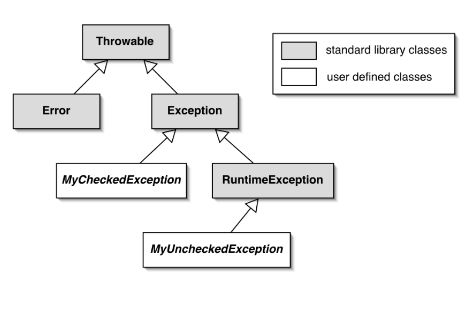
\includegraphics[height=7cm, keepaspectratio]{images/errors}
\end{center}
\end{frame}

\begin{frame}
\begin{center}
\textbf{java.lang.Error}
\end{center}
\begin{itemize}
\item Indicates serious problems that a reasonable application should not
try to catch
\item A method is not required to declare in its throws clause any
subclasses of Error
\end{itemize}
\end{frame}

\begin{frame}
\begin{center}
\textbf{Checked Exceptions - java.lang.Exception}
\end{center}
\begin{itemize}
\item Checked exceptions Subclass of Exception
\begin{itemize}
\item Use for anticipated failures. 
\item Where recovery may be possible.
\end{itemize}
\bigskip
\item Checked exceptions must be caught in your code \\- compiler enforces it
\item e.g. readLine() throws a IOException which must be caught
\end{itemize}
\end{frame}

\begin{frame}
\begin{center}
\textbf{The Effect of An Exception}
\end{center}
\begin{itemize}
\item The throwing method finishes prematurely.
\item No return value is returned.
\item Control does not return to the clients point of call.
\begin{itemize}
\item So the client cannot carry on regardless. 
\end{itemize}
\item A client may catch an exception.
\end{itemize}
\end{frame}

\begin{frame}
\begin{center}
\textbf{Unchecked Exceptions - java.lang.RuntimeException}
\end{center}
\begin{itemize}
\item Use of these is unchecked by the compiler. 
\item Cause program termination if not caught.
\begin{itemize}
\item This is the normal practice. 
\end{itemize}
\item IllegalArgumentException is a typical example.
\end{itemize}
\end{frame}

\begin{frame}
\begin{center}
\textbf{Runtime Exception}
\end{center}
\begin{itemize}
\item The next question might be: 
\item If it's so good to document a method's API, including the exceptions it can throw, why not specify runtime exceptions too? 
\item Runtime exceptions represent problems that are the result of a programming problem, and as such, the API client code cannot reasonably be expected to recover from them or to handle them in any way. 
\item Such problems include:
\begin{itemize}
\item arithmetic exceptions, such as dividing by zero
\item pointer exceptions, such as trying to access an object through a null reference 
\item and indexing exceptions, such as attempting to access an array element through an index that is too large or too small.
\end{itemize}
\end{itemize}
\end{frame}

\begin{frame}[fragile]
\begin{center}
\textbf{Argument Checking}
\end{center}
\begin{block}{}
\begin{lstlisting}
public ContactDetails getDetails (String key){
  if(key == null){
    throw new NullPointerException
        ("null key in getDetails"); 
  }
  
  if(key.trim().length() == 0){
    throw new IllegalArgumentException
         ("Empty key passed to getDetails");
   }  
   
  return book.get(key);
}
\end{lstlisting}
\end{block}
\end{frame}

\begin{frame}[fragile]
\begin{center}
\textbf{Preventing Object Creation}
\end{center}
\begin{block}{}
\begin{lstlisting}
public ContactDetails newDetails (String name){
  if(name == null){
    throw new NullPointerException
        ("null name in newDetails"); 
  }
  
  if(name.trim().length() == 0){
    throw new IllegalArgumentException
         ("Empty name passed to newDetails");
   }  
   
  return new ContactDetails(name);
}
\end{lstlisting}
\end{block}
\end{frame}

\begin{frame}
\begin{center}
\textbf{Exception Handling}
\end{center}
\begin{itemize}
\item Checked exceptions are meant to be caught.
\item The compiler ensures that their use is tightly controlled.
\begin{itemize}
\item In both server and client.
\end{itemize}
\item Used properly, failures may be recoverable.
\end{itemize}
\end{frame}


\begin{frame}[fragile]
\begin{center}
\textbf{The Throws Clause}
\end{center}
\begin{itemize}
\item Methods throwing a checked exception must include a throws clause:
\end{itemize}

\begin{block}{}
\begin{lstlisting}
public void saveToFile(String destinationFile) 
         throws IOException
\end{lstlisting}
\end{block}
\end{frame}

\begin{frame}[fragile]
\begin{center}
\textbf{The Try Block}
\end{center}
\begin{itemize}
\item Clients catching an exception must protect the call with a try block:
\end{itemize}
\begin{block}{}
\begin{lstlisting}
  try{
    Protect one or more statements here .
  }
  catch(IOException e){
    Report and recover from  exception here.
  }
\end{lstlisting}
\end{block}
\end{frame}

\begin{frame}[fragile]
\begin{center}
\textbf{The Try Block}
\end{center}
\begin{block}{}
\begin{lstlisting}
try{
  addressbook.saveToFile(filename); 
  tryAgain = false;
}
catch(IOException e) {
  System.out.println("Unable to save to " + filename);
  tryAgain = true; 
}
\end{lstlisting}
\end{block}
\end{frame}

\begin{frame}[fragile]
\begin{center}
\textbf{Checking Multiple Exceptions}
\end{center}
\begin{block}{}
\begin{lstlisting}
try{
  ...
  ref.process() ;
  ...
}
catch (EOFException e){
  // Take action on an end-of-file exception
  ...
}
catch(FileNotFoundException e) {
  //Take action on a file-not-found exception
   ...
}
\end{lstlisting}
\end{block}

\end{frame}

\begin{frame}[fragile] 
\begin{center}
\textbf{Finally}
\end{center}
\begin{block}{}
\begin{lstlisting}
  try{
    Protect one or more statements here .
  }
  catch(Exception e){
    Report and recover from  exception here.
  }
  finally{
    Perform any actions here that must occur 
    whether or not an exception is thrown
  }
\end{lstlisting}
\end{block}
\end{frame}

\begin{frame}
\begin{center}
\textbf{The Finally Clause}
\end{center}
\begin{itemize}
\item A finally clause is executed even if a return statement is executed in the try or catch clauses.
\item A uncaught or propagated exception still exits via the finally clause.
\end{itemize} 
\end{frame}

\begin{frame}
\begin{center}
\textbf{FileWriter: an Example}
\end{center}
\begin{itemize}
\item Use the FileWriter class. 
\begin{itemize}
\item Open a file.
\item Write to the file. 
\item Close the file.
\end{itemize}
\item Failure at any point results in an IOException.
\end{itemize}
\end{frame}

\begin{frame}[fragile]
\begin{block}{}
\begin{lstlisting}
try {
  FileWriter writer = new FileWriter(name of file��); 
  while ( there is more text to write ){
    ...
    writer.write(next piece of text)
    ...
}
catch(IOException e){
  something went wrong with accessing the file
}
finally{
  writer.close();	
}
\end{lstlisting}
\end{block}
\end{frame}

\begin{frame}
\begin{center}
\textbf{Defining New Exceptions}
\end{center}
\begin{itemize}
\item Extend Exception or RuntimeException.
\item Define new types to give better diagnostic information. 
\item Include reporting and/or recovery information.
\end{itemize}
\end{frame}

\begin{frame}[fragile]
\begin{block}{}
\begin{lstlisting}
public class NoMatchingDetailsException 
                     extends Exception{

  private String key;

  public NoMatchingDetailsException(String key){
    this.key=key;
  }

  public String getKey(){
    return key;	
  }

  public String toString(){
    return "No details matching"+ key +"found";
  }
}
\end{lstlisting}
\end{block}
\end{frame}

\begin{frame}[fragile]
\begin{block}{}
\begin{lstlisting}
public class AddressBook{
    
    HashMap<Integer, ContactDetails> mycontacts;
    
    public ContactDetails get(String key) 
        throws NoMatchingDetailsException{
          
        ContactDetails cd = mycontacts.get(key);
        if(cd == null){
            throw new NoMatchingDetailsException("Unknown Contact"); 
        }
        return cd;
    }
}
\end{lstlisting}
\end{block}
\end{frame}

\begin{frame}[fragile]
\begin{block}{}
\begin{lstlisting}
public ContactDetails getDetails (String key){
  
    if(key == null){
        throw new NullPointerException("null key in getDetails"); 
    }
  
    if(key.trim().length() == 0){
        throw new IllegalArgumentException("Empty key passed to getDetails");
    }  
    
    try{
        return book.get(key);
    }
    catch(NoMatchingDetailsException e){
        // recovery code
    }
}
\end{lstlisting}
\end{block}
\end{frame}

\section{Assertions}

\begin{frame}
\begin{center}
\textbf{Assertions}
\end{center}
\begin{itemize}
\item Used for internal consistency checks. 
\begin{itemize}
\item e.g. object state following mutation.
\end{itemize}
\bigskip
\item Used during development and normally removed in production version.
\begin{itemize}
\item e.g. via a compile-time option. 
\end{itemize}
\end{itemize}
\end{frame}

\begin{frame}
\begin{center}
\textbf{The Java Assertion Statement}
\end{center}
\begin{itemize}
\item Two forms available:
\item assert boolean$-$expression
\item assert boolean$-$expression : expression2
\item The boolean-expression expresses something that should be true at this point.
\item An AssertionError is thrown if the assertion is false.
\item The second expression (expression2) is a detailed error message that is passed to the AssertionError (and then to the user).
\end{itemize}
\end{frame}

\begin{frame}[fragile]
\begin{block}{}
\begin{lstlisting}
//Assert Statement
public void removeDetails(String key){
  if(key == null){
    throw new IllegalArgumentException (". . . ") ;
  }
  if (keyInUse(key) ) {
    ContactDetails details = book.get(key); 
    book.remove(details.getName() ) ; 
    book.remove(details.getPhone() ) ; 
    numberOfEntries --;
  }
  assert !keyInUse(key); 
  assert consistentSize () :
        "Inconsistent book size in removeDetails";
}
\end{lstlisting}
\end{block}
\end{frame}

\begin{frame}[fragile]
\begin{center}
\textbf{Guidelines for Assertions}
\end{center}
\begin{itemize}
\item They are not an alternative to throwing exceptions. 
\item Use for internal checks.
\item Remove from production code.
\item Do not include normal functionality:
\end{itemize}

\begin{block}{}
\begin{lstlisting}
//Incorrect Use
assert book.remove(name) != null;
\end{lstlisting}
\end{block}
\end{frame}

\begin{frame}[fragile]
\begin{itemize}
\item In order to use assertions in your pre-production code...
\item ... compile using the - -source 1.4 switch
\item ... run using the - -ea switch
\end{itemize}

\begin{block}{}
\begin{lstlisting}
$ javac --source 1.4 MyClass.java

$ java --ea MyClass
\end{lstlisting}
\end{block}

\begin{itemize}
\item For more information, see the Java tutorial
\end{itemize}
\begin{center}
\small
http://docs.oracle.com/javase/8/docs/technotes/guides/language/assert.html
\end{center}
\end{frame}

\section{Error Recovery}

\begin{frame}
\begin{center}
\textbf{Error Recovery}
\end{center}
\begin{itemize}
\item Clients should take note of error notifications. 
\item Check return values.
\item Do not ignore exceptions.
\item Include code to attempt recovery. 
\item Will often require a loop.
\end{itemize}
\end{frame}

\begin{frame}[fragile]
\begin{block}{}
\begin{lstlisting}
boolean successful=false;
int attempts = 0;

while (!successful && attempts<MAX_ATTEMPTS) {
  try {
    addressbook.saveToFile(filename); 
    successful = true ;
  }
  catch(IOException e) {
    System.out.println("Error saving�� " + filename); 
    attempts ++;
    if(attempts < MAX_ATTEMPTS) {
      filename = an alternative file name;
    } 
  }
} 

if(!successful){
  Report the problem and give up ;
}
\end{lstlisting}
\end{block}
\end{frame}

\begin{frame}
\begin{center}
\textbf{Error Avoidance}
\end{center}
\begin{itemize}
\item Clients can often use server query methods to avoid errors.
\begin{itemize}
\item More robust clients mean servers can be more trusting. 
\item Unchecked exceptions can be used.
\item Simplifies client logic.
\end{itemize}
\item May increase client-server coupling.
\end{itemize}
\end{frame}

\begin{frame}[fragile]
\begin{center}
\textbf{Avoiding An Exception}
\end{center}
\begin{block}{}
\begin{lstlisting}
// use the correct method to put details
// in the address book.
if (book.keyInUse( details .getName() ||
      book.keyInUse(details.getPhone()){
  book.changeDetails(details);
}
else{
  book.addDetails(details);
}
\end{lstlisting}
\end{block}
\end{frame}

\begin{frame}
\begin{center}
\textbf{Review}
\end{center}
\begin{itemize}
\item Runtime errors arise for many reasons.
\begin{itemize}
\item An inappropriate client call to a server object.
\item A server unable to fulfil a request. 
\item Programming error in client and/or server.
\end{itemize}
\item Runtime errors often lead to program failure.
\item Defensive programming anticipates errors in both client and server.
\item Exceptions provide a reporting and recovery mechanism.
\end{itemize}
\end{frame}

\begin{frame}
\begin{itemize}
\item Input/Output Errors
\item Input-output is particularly error-prone.
\item It involves interaction with the external environment. 
\item The java.io package supports input-output. 
\item java.io.IOException is a checked exception.
\end{itemize}
\end{frame}

\section{Style : Writing Better Code}

\begin{frame}
\begin{center}
\textbf{Style : Writing Better Code}
\end{center}
\begin{itemize}
\item Maintainance 
\item Coupling - Cohesion 
\item Improving Code 
\end{itemize}
\end{frame}

\begin{frame}
\begin{center}
\textbf{Software Changes}
\end{center}
\begin{itemize}
\item Software is not like a novel that is written once and then remains unchanged.
\item Software is extended, corrected, maintained, ported, adapted
\item The work is done by different people over time (often decades).
\end{itemize}
\end{frame}

\begin{frame}
\begin{itemize}
\item Change or Become Useless!
\item There are only two options for software: 
\begin{itemize}
\item Either it is continuously maintained
\item Or it becomes useless.
\end{itemize}
\item Software that cannot be maintained will be thrown away.
\end{itemize}
\end{frame}

\begin{frame}
\begin{center}
\textbf{Code Quality}
\end{center}
\begin{itemize}
\item Two important concepts for quality of evolving code:
\bigskip
\item Coupling 
\item Cohesion
\end{itemize}
\end{frame}

\begin{frame}
\begin{center}
\textbf{Coupling}
\end{center}
\begin{itemize}
\item Coupling refers to links between separate units of a program.
\item If two classes depend closely on many details of each other, we say they are tightly coupled.
\item Aim for loose coupling.
\end{itemize}
\end{frame}

\begin{frame}
\begin{center}
\textbf{Loose Coupling}
\end{center}
\begin{itemize}
\item Loose coupling makes it possible to:
\begin{itemize}
\item understand one class without reading others
\item change one class without affecting others
\end{itemize}
\item Thus: improves maintainability.
\end{itemize}
\end{frame}

\begin{frame}
\begin{center}
\textbf{Cohesion}
\end{center}
\begin{itemize}
\item Cohesion refers to the the number and diversity of tasks that a single unit is responsible for.
\item If each unit is responsible for one single logical task, we say it has high cohesion.
\item Cohesion applies to classes and methods. 
\item Aim for high cohesion.
\end{itemize}
\end{frame}

\begin{frame}
\begin{center}
\textbf{High Cohesion}
\end{center}
\begin{itemize}
\item High cohesion makes it easier to:
\bigskip
\item Understand what a class or method does
\item Use descriptive names
\item Reuse classes or methods
\end{itemize}
\end{frame}

\begin{frame}
\begin{center}
\textbf{Cohesion of Methods}
\end{center}
\begin{itemize}
\item A method should be responsible for one and only one well defined task
\end{itemize}
\end{frame}

\begin{frame}
\begin{center}
\textbf{Cohesion of Classes}
\end{center}
\begin{itemize}
\item Classes should represent one single, well defined entity.
\end{itemize}
\end{frame}

\begin{frame}
\begin{center}
\textbf{Code Duplication}
\end{center}
\begin{itemize}
\item Is an indicator of bad design,
\item Makes maintenance harder,
\item Can lead to introduction of errors during maintenance.
\end{itemize}
\end{frame}

\begin{frame}
\begin{center}
\textbf{Responsibility-Driven Design}
\end{center}
\begin{itemize}
\item Question: where should we add a new method (which class)?
\item Each class should be responsible for manipulating its own data.
\item The class that owns the data should be responsible for processing it.
\item Responsibility-driven design leads to low coupling.
\end{itemize}
\end{frame}

\begin{frame}
\begin{center}
\textbf{Localising Change}
\end{center}
\begin{itemize}
\item One aim of reducing coupling and responsibility-driven design is to localize change.
\item When a change is needed, as few classes as possible should be affected.
\end{itemize}
\end{frame}

\begin{frame}
\begin{center}
\textbf{Thinking Ahead}
\end{center}
\begin{itemize}
\item When designing a class, we try to think what changes are likely to be made in the future.
\item We aim to make those changes easy.
\end{itemize}
\end{frame}

\begin{frame}
\begin{center}
\textbf{Refactoring}
\end{center}
\begin{itemize}
\item When classes are maintained, often code is added. 
\item Classes and methods tend to become longer.
\item Every now and then, classes and methods should be refactored to maintain cohesion and low coupling.
\end{itemize}
\end{frame}

\begin{frame}
\begin{center}
\textbf{Refactoring and Testing}
\end{center}
\begin{itemize}
\item When refactoring code, separate the refactoring from making other changes.
\item First do the refactoring only, without changing the functionality.
\item Test before and after refactoring to ensure that nothing was broken.
\end{itemize}
\end{frame}

\begin{frame}
\begin{center}
\textbf{Design Questions}
\end{center}
\begin{itemize}
\item Common questions
\begin{itemize}
\item How long should a class be?
\item How long should a method be?
\end{itemize}
\item Can now be answered in terms of cohesion and coupling
\end{itemize}
\end{frame}

\begin{frame}
\begin{center}
\textbf{Design Guidelines}
\end{center}
\begin{itemize}
\item A method is too long if it does more then one logical task.
\item A class is too complex if it represents more than one logical entity.
\item Note these are guidelines. They still leave much open to the designer
% \item We will look at these guidelines in more detail in this afternoon's lecture
\end{itemize}
\end{frame}

\end{document}